Explain the project and what we want to accomplish.

\section{Atkinson and Sack algorithm}
Describe briefly the algorithm here.

\section{Implementation using R}

\begin{lstlisting}
  generate.tree <- function(number_of_nodes){
    word_dimension <- 2 * number_of_nodes    
    universe <- 1:word_dimension
    sample <- sample(universe, size=number_of_nodes)
    w = rep(0, word_dimension)
    for (i in 1:word_dimension) {
      w[i] <- ifelse(any(sample == i), 1, -1)
    }    
    phi=phi(w)
    list(word=w, phi=phi, as_brackets = brackets_of_word(phi))
  }

  split.word <- function(w){
    if(length(w) == 0){
      return(list(u=c(), v=c()))
    }    
    u_index_set <- 1:match(0, cumsum(w))
    list(u=w[u_index_set], v=w[-u_index_set])
  }

  phi <- function(w){
    if(length(w) == 0){
      return(w)
    }    
    split <- split.word(w)     
    if(all(cumsum(split$u) > -1)){
      return (c(split$u, phi(split$v)))
    }
    else{
      t = split$u[-c(1, length(split$u))]
      return (c(1, phi(split$v), -1, -t))
    }
  }
\end{lstlisting}

% latex table generated in R 2.15.1 by xtable 1.5-6 package
% Sun Dec 23 17:49:56 2012
\begin{table}[ht]
\begin{center}
\begin{tabular}{rrrrrr}
  \hline
  number\_of\_nodes & 4 & 5 & 6 & 8 & 10 \\ 
  number\_of\_trees & 14 & 42 & 132 & 1430 & 16796 \\ 
  \hline
\end{tabular}
\end{center}
\end{table}
% latex table generated in R 2.15.1 by xtable 1.5-6 package
% Sun Dec 23 17:49:56 2012
\begin{table}[ht]
\begin{center}
\begin{tabular}{rrrrrr}
  \hline
 & 4 & 5 & 6 & 8 & 10 \\ 
  \hline
1000 & 0.60 & 0.85 & 0.54 & 1.00 & 1.00 \\ 
  2000 & 0.99 & 0.98 & 0.13 & 1.00 & 1.00 \\ 
  5000 & 0.36 & 0.85 & 0.28 & 1.00 & 1.00 \\ 
  10000 & 0.69 & 0.73 & 0.11 & 0.65 & 1.00 \\ 
  20000 & 0.63 & 0.23 & 0.50 & 0.16 & 1.00 \\ 
  50000 & 0.09 & 0.74 & 0.63 & 0.90 & 1.00 \\ 
   \hline
\end{tabular}
\end{center}
\end{table}
% latex table generated in R 2.15.1 by xtable 1.5-6 package
% Sun Dec 23 17:49:56 2012
\begin{table}[ht]
\begin{center}
\begin{tabular}{rrrrrr}
  \hline
 & 4 & 5 & 6 & 8 & 10 \\ 
  \hline
1000 & 11.08 & 31.69 & 128.86 & 1456.74 & 16770.17 \\ 
  2000 & 4.39 & 24.36 & 149.75 & 1454.88 & 17046.66 \\ 
  5000 & 14.18 & 31.62 & 140.13 & 1378.37 & 16478.72 \\ 
  10000 & 10.09 & 35.05 & 151.54 & 1414.26 & 17028.12 \\ 
  20000 & 10.75 & 47.34 & 130.37 & 1483.03 & 16813.47 \\ 
  50000 & 20.26 & 34.83 & 125.10 & 1359.54 & 16778.21 \\ 
   \hline
\end{tabular}
\end{center}
\end{table}


\noindent
%%%%%%%%%%%%%%%
%%% INPUT:
\begin{minipage}[t]{8ex}{\color{red}\bf
\begin{verbatim}
(%i178) 
\end{verbatim}}
\end{minipage}
\begin{minipage}[t]{\textwidth}{\color{blue}
\begin{verbatim}
fpprintprec:4$
leaves(n):=(n*(n+1))/(2*(2*n-1));
combineResult(n):=[n,leaves(n)]$
map(combineResult, makelist(n,n,1,10)),numer;
\end{verbatim}}
\end{minipage}
%%% OUTPUT:
\definecolor{labelcolor}{RGB}{100,0,0}
\begin{math}\displaystyle
\parbox{8ex}{\color{labelcolor}(\%o179) }
\mathrm{leaves}\left( n\right) :=\frac{n\,\left( n+1\right)
}{2\,\left( 2\,n-1\right) }
\end{math}\\
\begin{math}\displaystyle
\parbox{8ex}{\color{labelcolor}(\%o181) }
[[1,1],[2,1],[3,1.2],[4,1.429],[5,1.667],[6,1.909],[7,2.154],[8,2.4],[9,2.647],[10,2.895]]
\end{math}
%%%%%%%%%%%%%%%


The following plots are obtained repeating 1000 times the generation
of 500 trees each with 5 nodes.
\begin{figure}[htb]
  \centering
  \includegraphics[height=13cm,
  width=13cm]{pictures/repeated-sampling-leaves-mean.pdf}
  \caption{Binary trees with four nodes}
  \label{fig:binary-trees-with-four-nodes}
\end{figure}

\begin{figure}[htb]
  \centering
  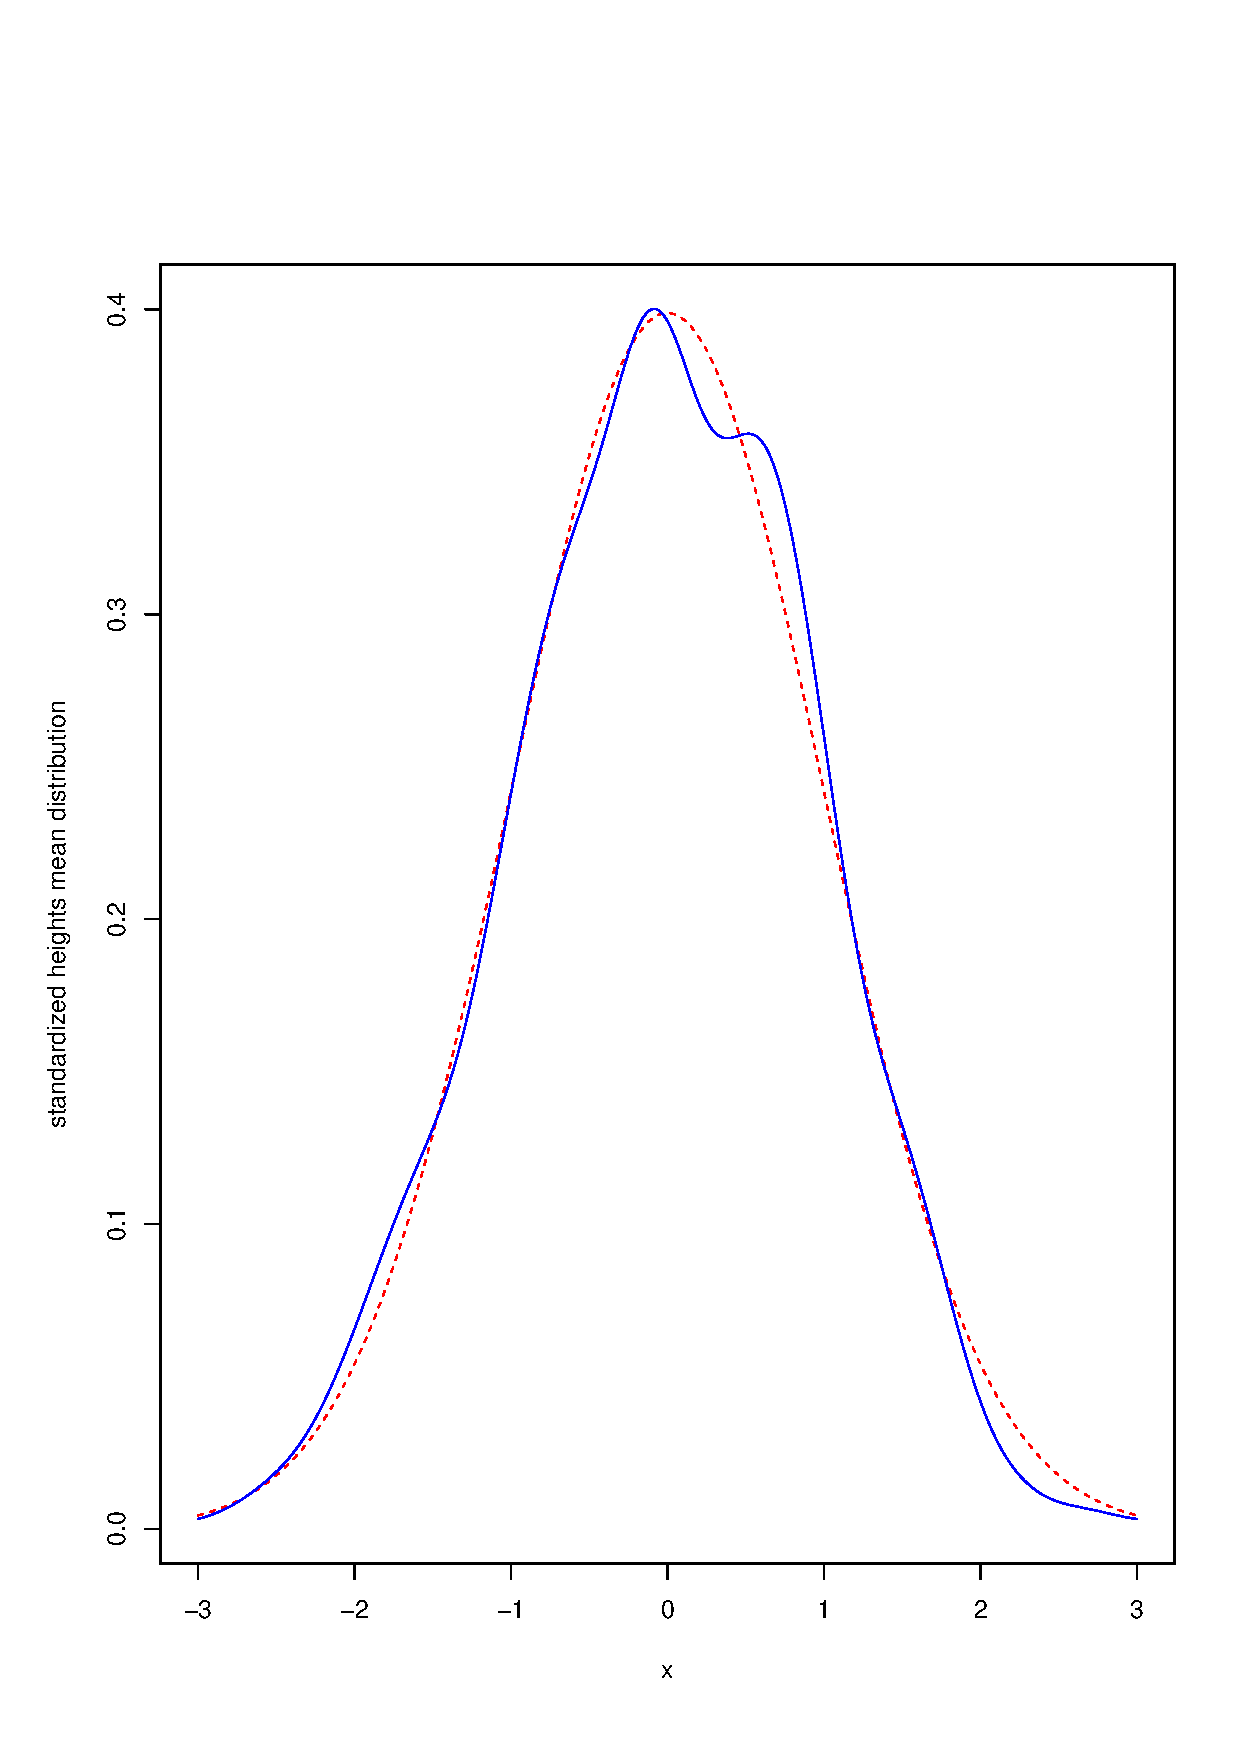
\includegraphics[height=13cm,
  width=13cm]{pictures/repeated-sampling-height-mean.pdf}
  \caption{Binary trees with four nodes}
  \label{fig:binary-trees-with-four-nodes}
\end{figure}


\begin{figure}[htb]
  \centering
  \rotatebox{90}{
    \includegraphics{pictures/binary-trees-with-four-nodes.png}
  }
  \caption{Binary trees with four nodes}
  \label{fig:binary-trees-with-four-nodes}
\end{figure}
